\documentclass{article}
\usepackage[a4paper]{geometry}
\usepackage[utf8]{inputenc}

\usepackage{graphicx}
\graphicspath{ {./images_P1/} }


\title{Informe pràctica 1\\Visió Artificial}
\author{Jordi Olivares Provencio\\Christian José Soler}

\begin{document}

\maketitle

\begin{enumerate}

 \item \textbf{Manipulación básica de imágenes}

 \begin{enumerate}

 \item \textit{Escribir una función (ej11()), que lee la imagen lena.jpg y la visualiza (figure,
imshow). ¿Qué tamaño tiene la imagen? Cuántos canales tiene? Convertir la
imagen en escala de grises (Help: rgb2gray) (Figura 1a). }

 La imagen tiene tamaño 225 x 225 y 3 canales.

 \item \textit{Obtener información sobre su tamaño (Help: mirar el workspace y el comando
size). Calcular el 10\% de su tamaño.}

 El 10\% son 23px

 \item \textit{“Incrustar” la imagen original en una imagen negra con un borde negro de
10\% de anchura/altura de la imagen original. ¿De qué tamaño ha de ser la
imagen negra?}

 La imagen negra ha de ser de tamaño (225 + 23*2) x (225 + 23*2) = 271 x 271

 \item \textit{Mostrar la imagen resultante y guardarla.}

 \begin{center}
 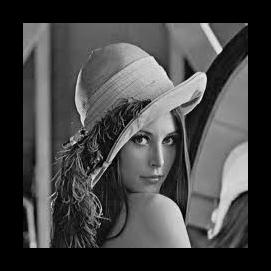
\includegraphics[width=0.5\textwidth]{lena_frame.jpg}
 \end{center}

 \end{enumerate}

\newpage

 \item \textbf{Cambios de color y contraste}

 \begin{enumerate}
 \item \textit{Crear la función ej12() que abre la imagen y la aclara de forma constante sin saturarla, de forma que el píxel más claro sea blanco (Figura 3 a)). Visualiza y compara el histograma (help: imhist()) de las dos imágenes y explica en qué se diferencian y en qué se parecen.}

 \begin{center}
 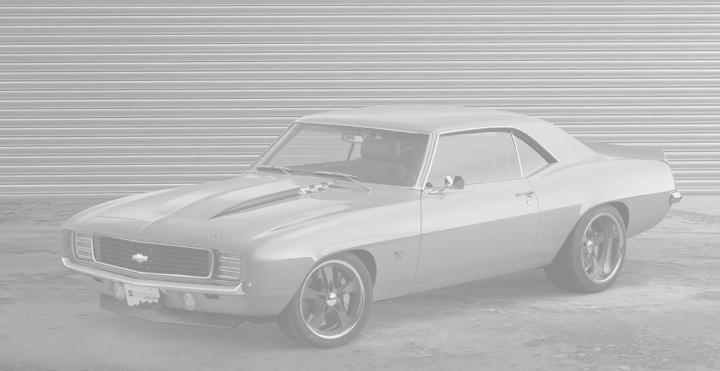
\includegraphics[width=0.4\textwidth]{car_bright.jpg}
 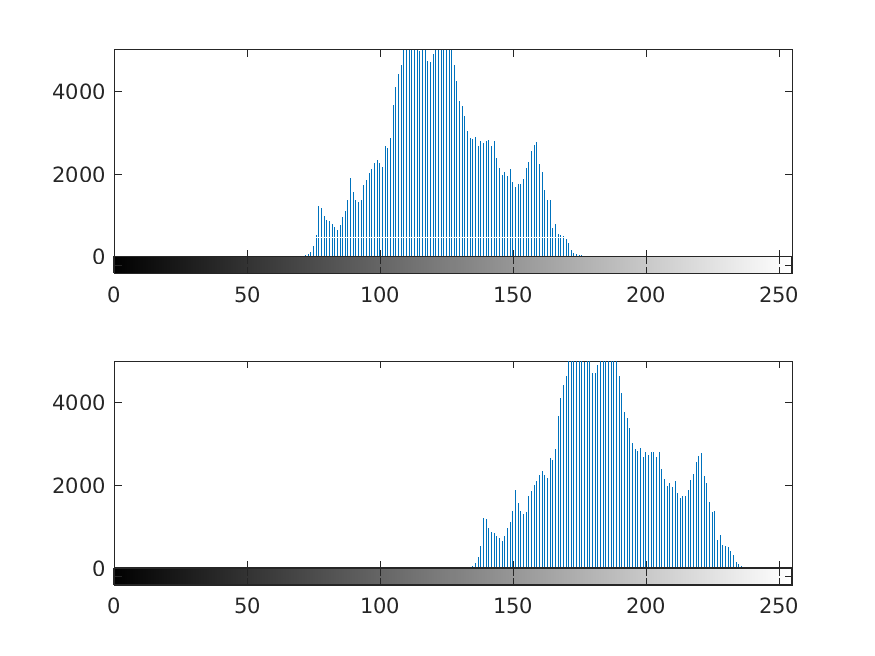
\includegraphics[width=0.6\textwidth]{subplot_2_high.png}
 \end{center}

 Son el mismo histograma con un desplazamiento a la derecha el modificado

 \item \textit{Abre la imagen y la oscurece de forma constante sin
saturarla, de forma que el píxel más oscuro sea negro (Figura 3 b)). Visualiza y compara el histograma (help: imhist()) de las dos imágenes y explica en qué se diferencian y en qué se parecen.}

 \begin{center}
 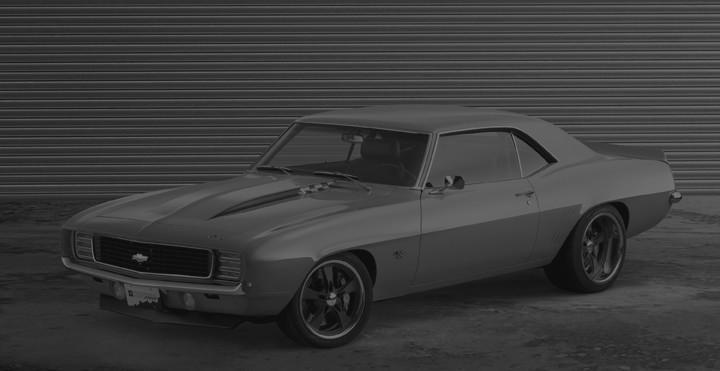
\includegraphics[width=0.4\textwidth]{car_dark.jpg}
 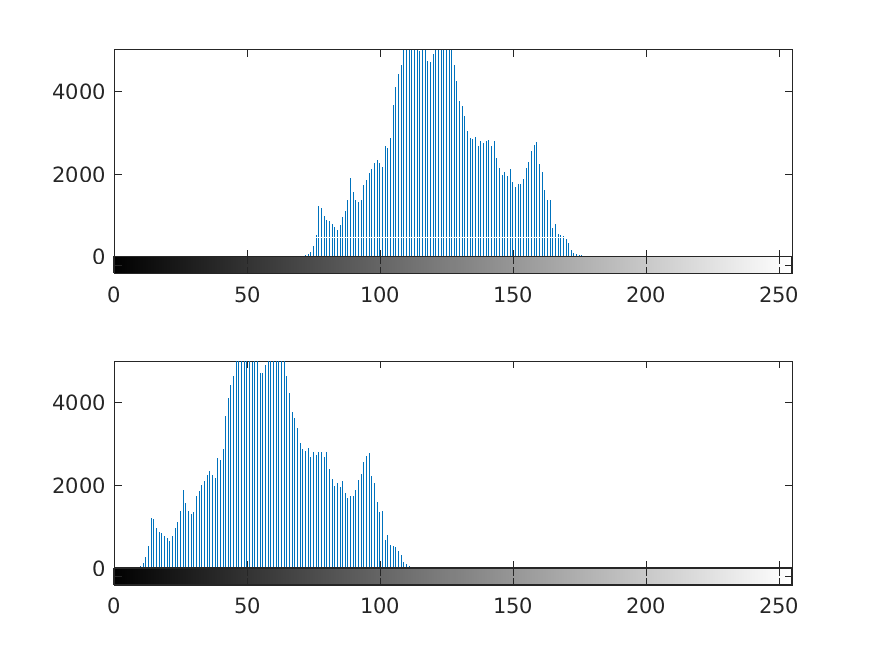
\includegraphics[width=0.6\textwidth]{subplot_2_low.png}
 \end{center}

 Son el mismo histograma con un desplazamiento a la izquierda el modificado

 \item \textit{A continuación aumenta el contraste de la imagen. Primeramente, abre la imagen y la convierte a tipo double con valores entre 0 y 1 (dividir todos los valores entre 255). Finalmente aumenta el contraste(Figura 3 c)). Visualiza y compara el histograma (help: imhist()) de las dos imágenes y explica en qué se diferencian y en qué se parecen.}

 \begin{center}
 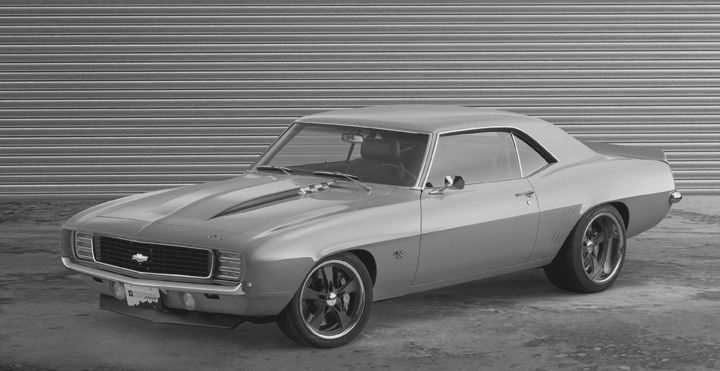
\includegraphics[width=0.4\textwidth]{car_contrast.jpg}
 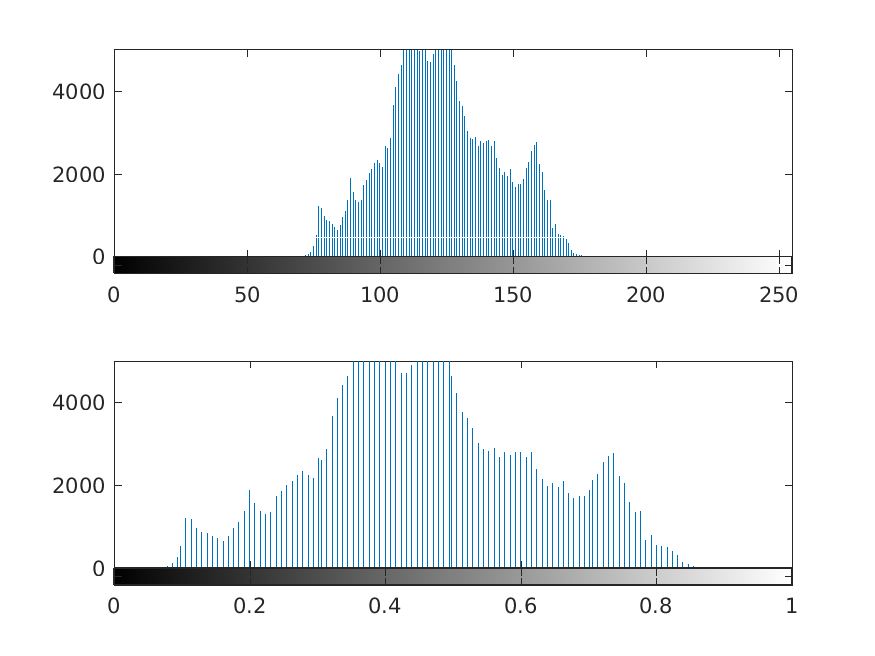
\includegraphics[width=0.6\textwidth]{subplot_2_contrast.png}
 \end{center}

 Son el mismo histograma, pero el modificado está extendido, para que ocupe todo el espectro.

 \end{enumerate}

\newpage

 \item \textbf{Binarización de imágenes}

 \begin{enumerate}
 \item \textit{Crea la versión binaria de la imagen original poniendo un umbral de
valor 130 y usando la indexación lógica. ¿Qué pasa si utilizamos un
valor de umbral diferente?¿Por qué? Modificar la función que se pueda
llamar con diferentes umbrales}

 Las partes no blancas, a medida que subimos el umbral, más partes quedan absorbidas directamente al color negro. Lo mismo al revés.

 \item \textit{Visualiza las dos imágenes en la misma figura}

 \begin{center}
 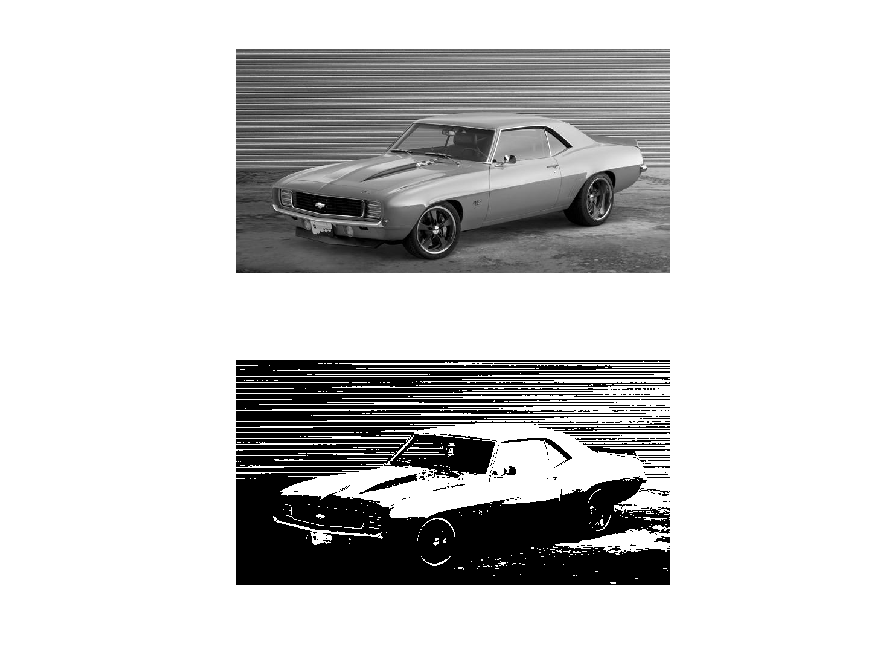
\includegraphics[width=0.5\textwidth]{subplot_3_binarize.png}
 \end{center}

 \item \textit{(opcional) Encuentra el comando de binarización (thresholding) en Matlab y
reimplementa con este comando la función ej13(). Help: puedes usar
el lookfor.}


 \end{enumerate}

\newpage

 \item \textbf{Trabajar con imágenes binarias y de escalas de gris}

 \begin{enumerate}
 \item \textit{Abrir la imagen circles.bmp, visualizarla y convertirla a escala de grises (Figura
6. a). Con imtool(im) puedes ver el valor de los píxeles de los círculos.}

 \item \textit{Crear 3 imágenes tipo binario a partir de la imagen inicial. En cada una de
ellas, se debe representar el fondo negro y cada uno de los 3 círculos en blanco
individualmente, utilizando los umbrales de valor correspondiente a los tres
círculos (Figura 6. b). Visualizar las tres imágenes en la misma figura usando el
subplot.}

 \begin{center}
 
\includegraphics[width=0.5\textwidth]{subplot_4_binary.png}
 \end{center}

 \item \textit{Utiliza las matrices binarias creadas en b) para generar 3 imágenes, donde
aparezcan cada uno de los círculos con su nivel de gris original. (Figura 6. c)}

 \begin{center}
 
\includegraphics[width=0.5\textwidth]{subplot_4_circles.png}
 \end{center}

 \end{enumerate}

\newpage

 \item \textbf{Visualización de imágenes en color}

 \begin{enumerate}
 \item \textit{Leer	la imagen. Visualizar los diferentes canales y explicar la diferencia entre los	valores de los píxeles. ¿Qué sucede si en la imagen en color intercambiamos los canales? ¿Qué sucede si en la imagen en color multiplicamos uno de los canales por 0?}

 \begin{center}
 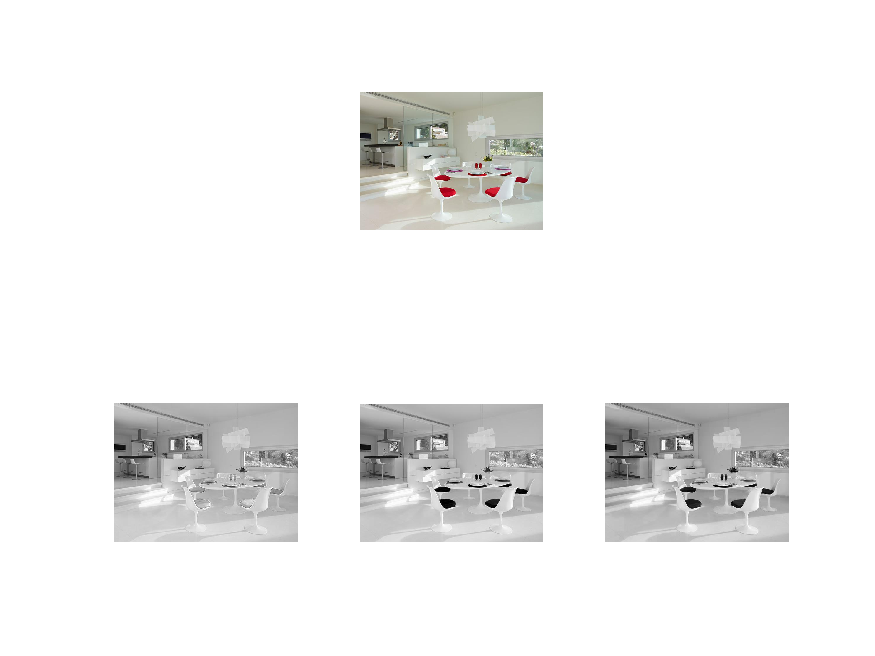
\includegraphics[width=0.8\textwidth]{subplot_5.png}
 \end{center}

 Ponemos el canal G = 0 y mostramos la imagen resultante

 \begin{center}
 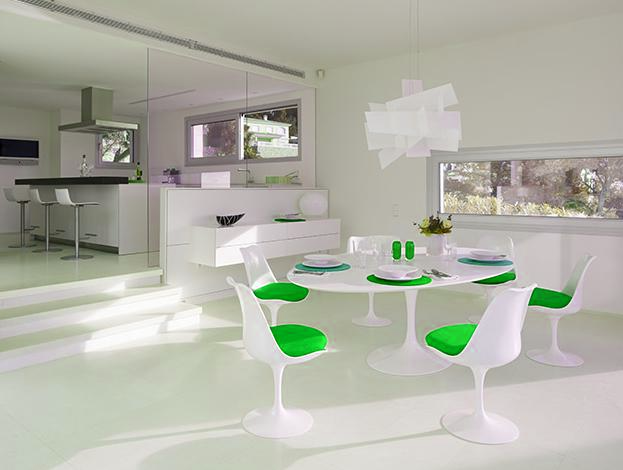
\includegraphics[width=0.5\textwidth]{ej15_cambiados.png}
 \end{center}


 \end{enumerate}

\newpage

 \item \textbf{Creación de imágenes de 3 canales (en color)}

 \begin{enumerate}
 \item \textit{Crea las 3 imágenes en escala de grises mostradas en la figura 8 (arriba).}
 \item \textit{Combina las 3 imágenes de forma que se obtenga la imagen mostrada en
la figura 8 (abajo).}

 \begin{center}
 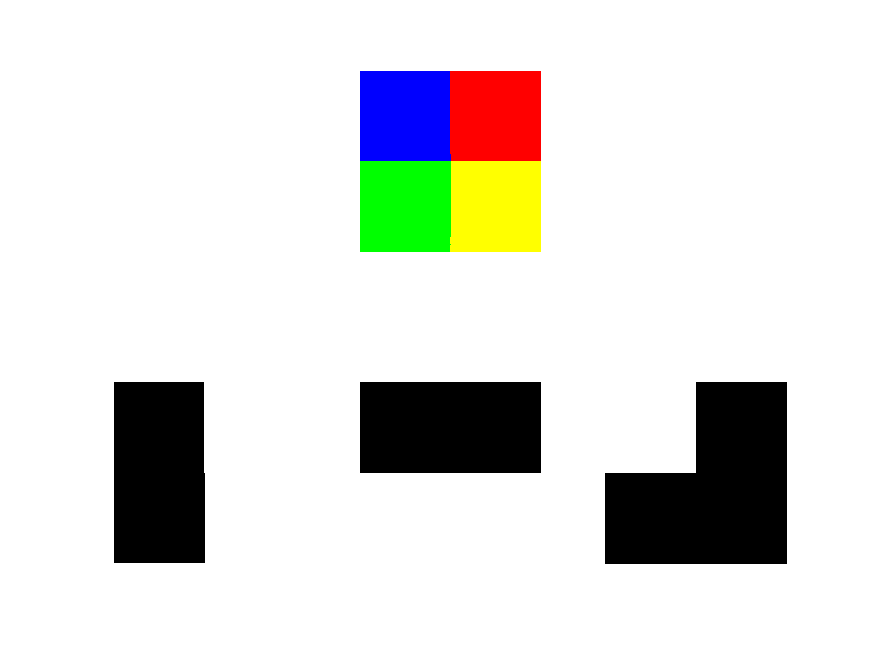
\includegraphics[width=0.5\textwidth]{subplot_6.png}
 \end{center}

 \item \textit{Guarda la imagen resultante como 3channels.jpg}

 \begin{center}
 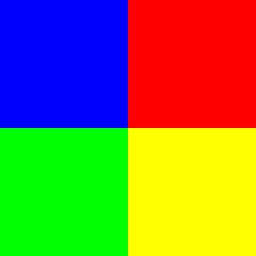
\includegraphics[width=0.5\textwidth]{3channels.jpg}
 \end{center}


 \end{enumerate}

\newpage

 \item \textbf{Tratamiento de imágenes en color RGB: modificación de una imagen}

 \begin{enumerate}
 \item \textit{Leer la imagen logo.png}
 \item \textit{Encontrar el vector de todos los pixeles que tiene color verde (6,118,85). Para
ello utilizar la función find.}
 \item \textit{Asignar a todos estos pixeles color rojo (255,0,0)}
 \item \textit{Visualizar las dos imágenes en una figura de la forma siguiente:}

 \begin{center}
 
\includegraphics[width=0.5\textwidth]{subplot_7.jpg}
 \end{center}

 \end{enumerate}

\newpage

 \item \textbf{Tratamiento de imágenes en color RGB}

 \begin{enumerate}
 \item \textit{Abrir los 2 archivos en MATLAB. ¿Cuántas dimensiones tienen las
imágenes?}

 coat.png - 1188 x 915 x 3 (3 dimensiones)

 model.png - 1188 x 915 x 3 (3 dimensiones)

 \item \textit{Convertir la imagen coat.png en escala de grises utilizando la función de
MATLAB apropiada.}

 \item \textit{Realizar una binarización sobre la imagen resultante en b) para conseguir
2 regiones: una perteneciente al abrigo (foreground) y la otra al fondo
(background). Crear otra imagen binaria invirtiendo las zonas de
foreground y background.}

 \item \textit{Utilizar las matrices binarias creadas en c) para fusionar las imágenes
model y coat (fig. 11 c).}

 \begin{center}
 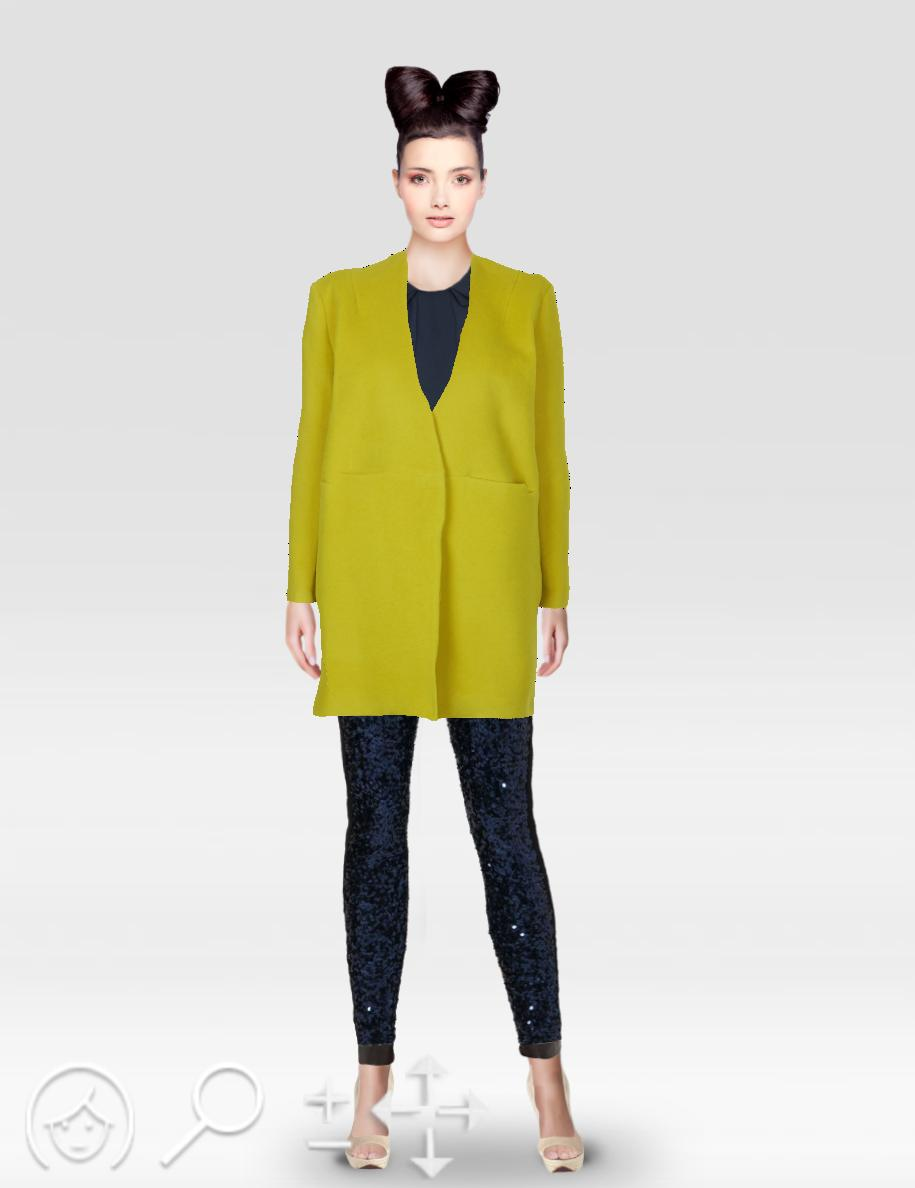
\includegraphics[width=0.2\textwidth]{model_coat.jpg}
 \end{center}

 \end{enumerate}

\end{enumerate}

\end{document}
